\documentclass[twoside,openright,a4paper,11pt,french]{article}
\usepackage[utf8]{inputenc}
\usepackage[french]{babel}
\usepackage[T1]{fontenc}
\usepackage{emptypage}
\usepackage{amsmath}

% Utilisation d'url
\usepackage{url}
\urlstyle{sf}

% Utilisation d'images, stockées dans le répertoire ./pics/
\usepackage{graphicx}
\graphicspath{pics/}

% Définition des marges
\usepackage{geometry}
\geometry{
  left=25mm,
  right=25mm,
  top=25mm,
  bottom=25mm,
  foot=15mm
}
\usepackage{listings}
\usepackage{color}

\definecolor{gray}{rgb}{0.8,0.8,0.8}

\begin{document}

\pagestyle{plain}
\setlength{\parindent}{0pt}
% La page de garde
\thispagestyle{empty}

\begin{center}
       \noindent
       
\includegraphics[height=2.5cm]{./pics/uds.eps}       
       
       \vfill\vfill

    {\large \textsc{Licence 3 de Sciences, mention Informatique}}

    \bigskip\bigskip

    {\large \textsc{Programmation Orientée Objet 2 }}

    \vfill\vfill

% Titre du document
    {\huge \sc
      \begin{center} 
        Rapport sur le projet: \\
        détection des bords et vectorisation
      \end{center}}

    \vfill\vfill

    {\large Présenté par}

\medskip

% Identité des auteurs
    {\large Victor \textsc{Constans}}\\
    {\large Luigi  \textsc{Coniglio}}\\
\bigskip

\end{center}



% La table des matières
\parskip=0pt
\tableofcontents


\vspace{5cm}

%Start content

\section{Fichiers rendus et usage}
\subsection{Contenu du rapport}
L'objectif de ce rapport est d'abord d'illustrer la structure du
programme. Pour accelérer/simplifier l'utilisation du travail rendu, la partie
initiale de ce rapport décrit le contenu des fichiers et leur usage.

\subsection{Contenu de l'archive}
Après avoir ouvert l'archive {\it constans\_coniglio\_luigi.tar.gz} vous
trouverez les fichiers et répertoires suivants:
\smallbreak
\begin{itemize}
\item Ce rapport
\item Le fichier {\bf javimy.java} qui est le point d'entrée du programme
\item Le répertoire {\bf gui} qui contient tous les fichiers du programme relatifs
      à l'interface graphique
\item Le répertoire {\bf filters} qui contient un package incluant tous les filtres 
      implementés dans la cadre de ce projet
\item Le répertoire {\bf vectorization} qui contient la partie du programme dédiée à
      la vectorisation d'une image
\end{itemize}

\bigbreak

\subsection{Usage}
Compiler le programme par le biais de la commande : 
\colorbox{gray}{\lstinline[basicstyle=\ttfamily\color{black}]| javac javimy.java |}
Une fois la création des fichiers{\it .class} terminé vous êtes prêt
à utiliser ce magnifigue logiciel: 
\colorbox{gray}{\lstinline[basicstyle=\ttfamily\color{black}]| java javimy |},

\vspace{1cm}
A l'exécution, il vous sera présenté une interface graphique qui vous
permettra de facon assez intuitive d'accéder aux differentes fonctions
du programme:

\begin{center}
% TODO image GUI %
\end{center}

\newpage 

\section{Filtres}
\label{sec:filtres}

\subsection{Sobel, Prewitt, Roberts, etc...}
%TODO Description du principe de fonctionnement avec quelque image/example

\subsection{Canny}
%TODO

\subsection{Gauss}
%TODO Description du principe de fonctionnement avec quelque image/example

\subsection{Segmentation}
La segmentation a pour objectif de partitionner une image en sections
(ensembles de pixels) sur la base de leurs propriétés (couleurs,
intensité, ...). Dans le menu des filtres vous trouverez un bouton qui
vous permettra de réaliser ce type d'opération sur les couleurs
d'une image.

L'algoritme utilisé pour segmenter l'image est inspiré du
partitionnement en {\it K-moyennes} (ou {\it k-means clustering} en
anglais). Ce type de partitionnement consiste à sélectioner K couleurs
et à assigner à chaque pixel de l'image à la plus proche de ces couleurs.

\begin{figure}[h]
\centering
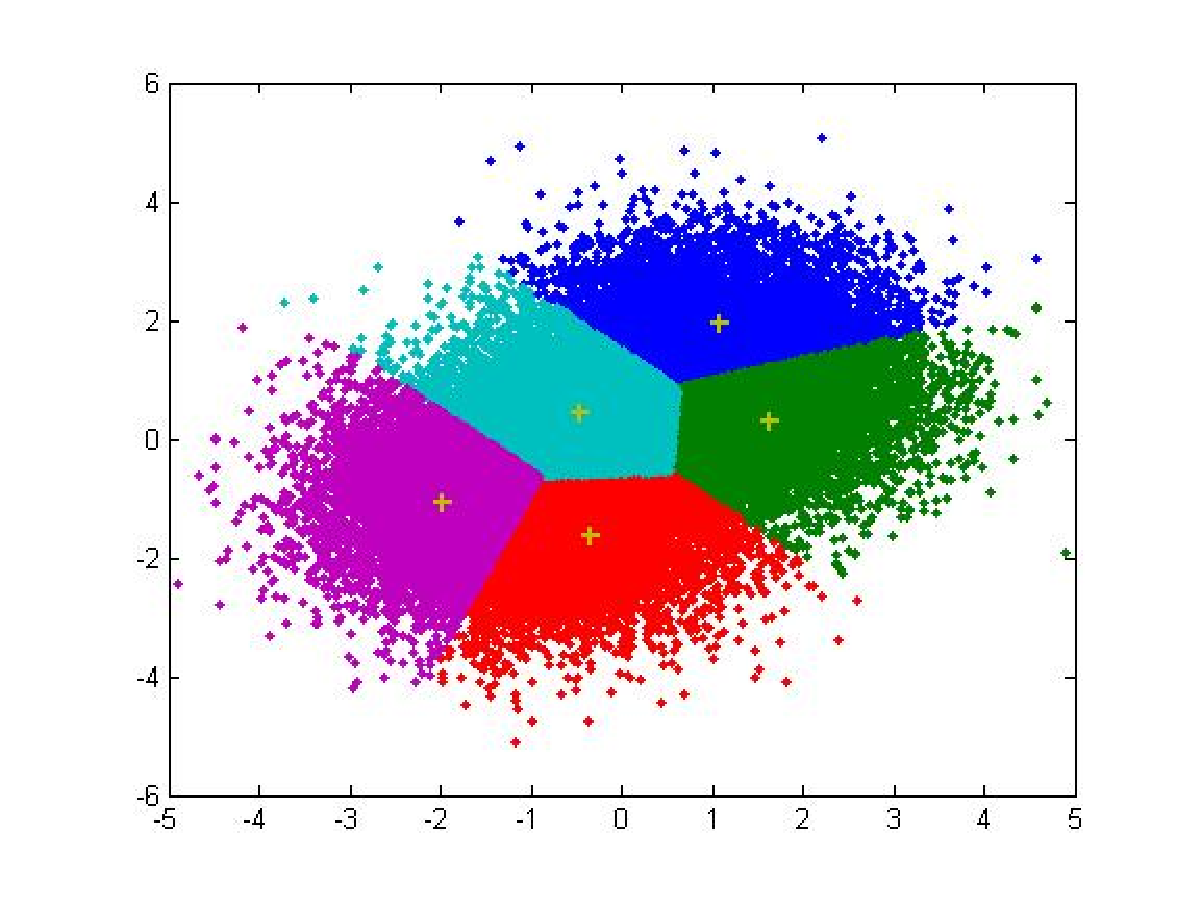
\includegraphics[width=8cm]{./pics/kmeans.eps}
\caption{Agrégation des pixels selon la plus courte distance avec les
K-moyennes (ici K = 5)}
\label{fig:routcidr}
\end{figure}

Les K couleurs vont ensuite êtres modifiées pour prendre comme valeur la
moyenne de la couleur des pixels qui lui sont associés, dans le but de
minimiser l'écart de couleur avec les pixels de l'image. Cette opération va
être répétée jusqu'à ce que les K couleurs et le partitionnement des pixels
convergent. 

\subsection{Cluster-edges}
Ce filtre s'inscrit dans l'ensemble des filtres de détections des
bords. La particularité de ce filtre vis-à-vis des autres filtres de
détection des contours est qu'il n'effectue pas qu'une simple détection
des bords mais. En effet, il détermine plus précisement les limites entre les
différentes zones de couleurs. 
La limite entre deux zones de couleurs est représentée par des
chemin coloré. A chaque bord correspond un chemin d'une couleur
différente \cite{url-novelvect}.

Le première étape de l'algoritme consiste à segmenter l'image en
différentes zones de couleurs.

\begin{figure}[h]
\centering
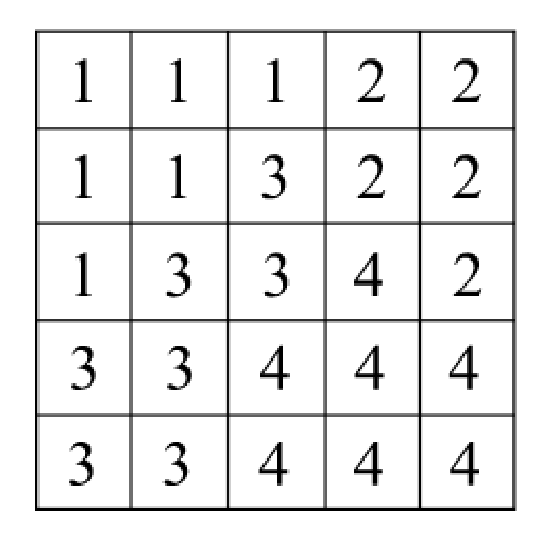
\includegraphics[width=3.5cm]{./pics/cluster-edges1.eps}
\caption{Segmentation, chaque nombre représente une couleur differente}
\label{fig:routcidr}
\end{figure}

Une fois la segmentation terminée on procède à la génération de
sub-pixels entre chaque pixel de l'image originale. Chaque sub-pixel
est rempli selon la couleur des pixels autour de lui.

\begin{figure}[h]
\centering
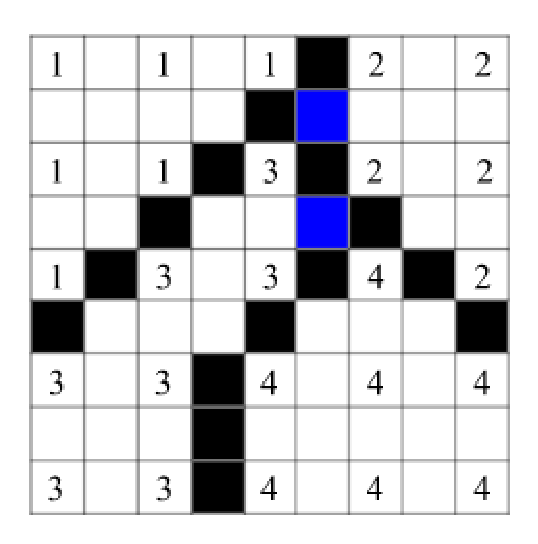
\includegraphics[width=3.5cm]{./pics/cluster-edges2.eps}
\caption{Les bords sont les sub-pixel ayant comme voisins des pixels de
couleur différente}
\label{fig:routcidr}
\end{figure}

\newpage

\section{Vectorisation} 
Le programme permet d'exporter une image sous la forme d'un fichier
{\it .svg}. La conversion d'une image dans le format SVG ({\it
Scalable Vector Graphics}) suit un processus assez complexe qui ne vaut
pas la peine d'être présenté.

Si la plupart des formats représentant une image en utilisant un 
mappage plus ou moins complexe de pixel, un format d'image vectorielle
permet de représenter une image comme etant un ensemble de formes
egendre par des vecteurs. Vectoriser une image consiste à traduire
l'ensemble des pixels d'une image en vecteurs (formes géométriques,
chemins, courbes, etc ...).

L'algorithme utilisé pour vectoriser une image dans le cadre de ce projet peut
être résumé par les étapes suivantes:   

\smallbreak
\begin{itemize}
\item Segmentation de l'image
\item Détection des contours et extraction des bords
\item Compression des bords
\item Construction des figures
\item Conversion au format SVG
\end{itemize}   
\bigbreak

La segmentation et la détection des contours d'une image sont effectuées
en utilisant les techiques présentes dans la section
\ref{sec:filtres} de ce rapport.


\subsection{Compression des bords}
%TODO Algorithme de Douglas-Peucker %
Au moment de la détection, chaque bord est extrait comme étant une
suite continue de pixels. Bien qu'une telle représentation soit tout à
fait utilisable dans la construction d'une image vectorielle le
resultat ne serait pas très différent de celui d'un format standard
d'image. C'est pour cette raison que pendant le processus de vectorisation d'une
image, les suites continues de pixels constituant les contours de
l'image doivent être traduits comme des éléments géométriques plus
simples: segments, courbes, etc.. .  

La première étape dans la traduction des contours consiste à réduire
le nombre de pixels. Dans la cadre de ce projet nous avons décidés d'utiliser
l'algorithme de Douglas-Peucker pour atteindre cet objectif
\cite{url-dougpeuck}.

L'algorithme de Douglas-Peucker est beaucoup utilisé en géographie
et permet d'approximer les points d'un chemin en tenant compte d'un
certain degré de liberté (paramétrable).

\begin{figure}[h]
\centering

\includegraphics[width=7cm]{./pics/dp1.eps}
\caption{Les bords sont approximés avec un degré de liberté croissant}
\label{fig:routcidr}
\end{figure}

Le fait que cet algorithme soit facilement paramétrable a été un élément clé
dans le choix de celui-ci, et il permet a l'utilisateur de choisir la précision
souhaité dans la vectorisation.

Un autre élément essentiel dans le choix de cet algorithme a été le
fait que il ne change pas la position du premier et du dernier point
d'un chemin dans la compression de celui-ci. Grâce à cela, un chemin
(partie d'un contour) d'une image commencera et terminera toujours sur
le en un même point, même après la compression, et assurant ainsi la
contiguité de celui-ci avec les bords voisins.



\subsection{Construction des figures}
%TODO voisinage de moore %
Une fois les contours simplifiés, arrive le moment de traiter
les zones de couleurs engendré par les bords.

On peut définire une {\it figure} comme étant une section de l'image ayant
(après segmentation) une unique couleur, et qui engendre la combinaison de
plusieurs bords.

Le but à ce stade est de détecter toutes les {\it figures} de l'image et
d'afféeter à chaque {\it figure} les bords entourant celle-ci dans le
bon ordre (sachant qu'un bord est toujours partagé entre deux
{\it figures}).

L'algorithme de construction des {\it figures} consiste à parcourir
l'image à la recherche des zones de couleur.

\begin{lstlisting}[frame=single]  % Start your code-block
Construction figures ( image )

Pixel p
Couleur c
Figure figures[]
Pour i=0...image.hauteur faire
    initialise c tel que c != image.pixel(i,0).couleur 
    Pour j=0...image.largeur faire
        si image.pixel(i,j).couleur != c et 
           image.pixel(i,j).traite = faux

            f <- image.pixel(i,j).extrait_figure()
            figures.ajouter(f)

            Pour tout pixel b dans f faire
                image.pixel(b.y,b.x).traite <- vrai
            fin 
        fin 
    fin
fin
renvoyer figures
\end{lstlisting}


Après avoir détecté une zone qui n'a pas encore été traitée, on procède
à l'examen des voisins \underline{externes} des pixels qui délimitent
la {\it figure}.

\begin{figure}[h]
\centering
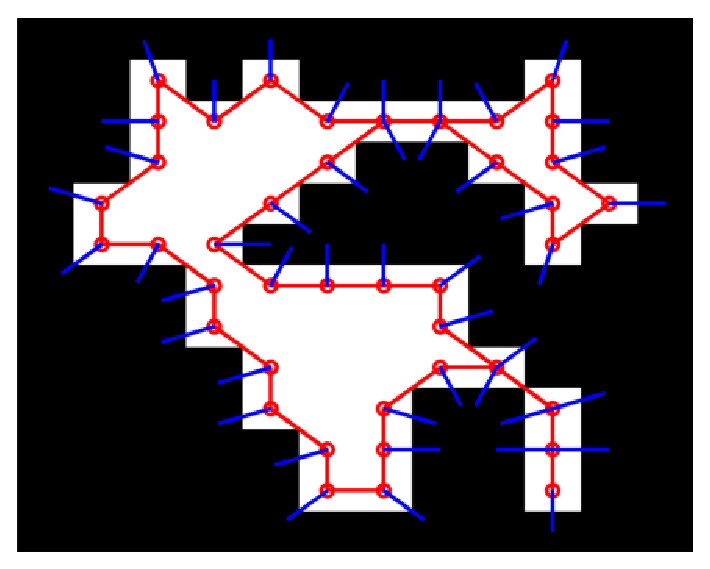
\includegraphics[width=7cm]{./pics/moore.eps}
\caption{Detection du voisinage externe d'une {\it figure}}
\label{fig:moore}
\end{figure}

Les contours d'une {\it figure} sont examine dans le sens horaire en
utilisant l'algoritme du voisinage de Moore \cite{url-moore}.




\section{Valeurs optimales}
%TODO valeurs optimales dans l'utilisation de chaque filtre%



\newpage
\addcontentsline{toc}{section}{Références}
\bibliographystyle{plain}
\bibliography{rapport}

\end{document}
